\documentclass[tikz,border=10pt]{standalone}
\usepackage{tikz}
\usetikzlibrary{shapes, arrows.meta, positioning, fit, calc}
\usepackage{soul}
\usepackage{textcomp}

% Define styles for nodes
\tikzset{
  level0/.style = {rectangle, draw=black, very thick, minimum width=3cm, minimum height=1cm, text centered, font=\sffamily\bfseries},
  level1/.style = {rectangle, rounded corners, draw=black, very thick, minimum width=1.5cm, minimum height=1cm, text centered, font=\sffamily\bfseries},
  level2/.style = {rectangle, draw=black, thick, minimum width=1.35cm, minimum height=1cm, text centered, font=\sffamily},
  level3/.style = {rectangle, rounded corners, draw=miamired, thick, font=\ttfamily, text=black, align=center, inner sep=2pt, minimum width=2cm, minimum height = .85cm}
}

% Define the 'miamired' color
\definecolor{miamired}{RGB}{200,16,46}

\begin{document}
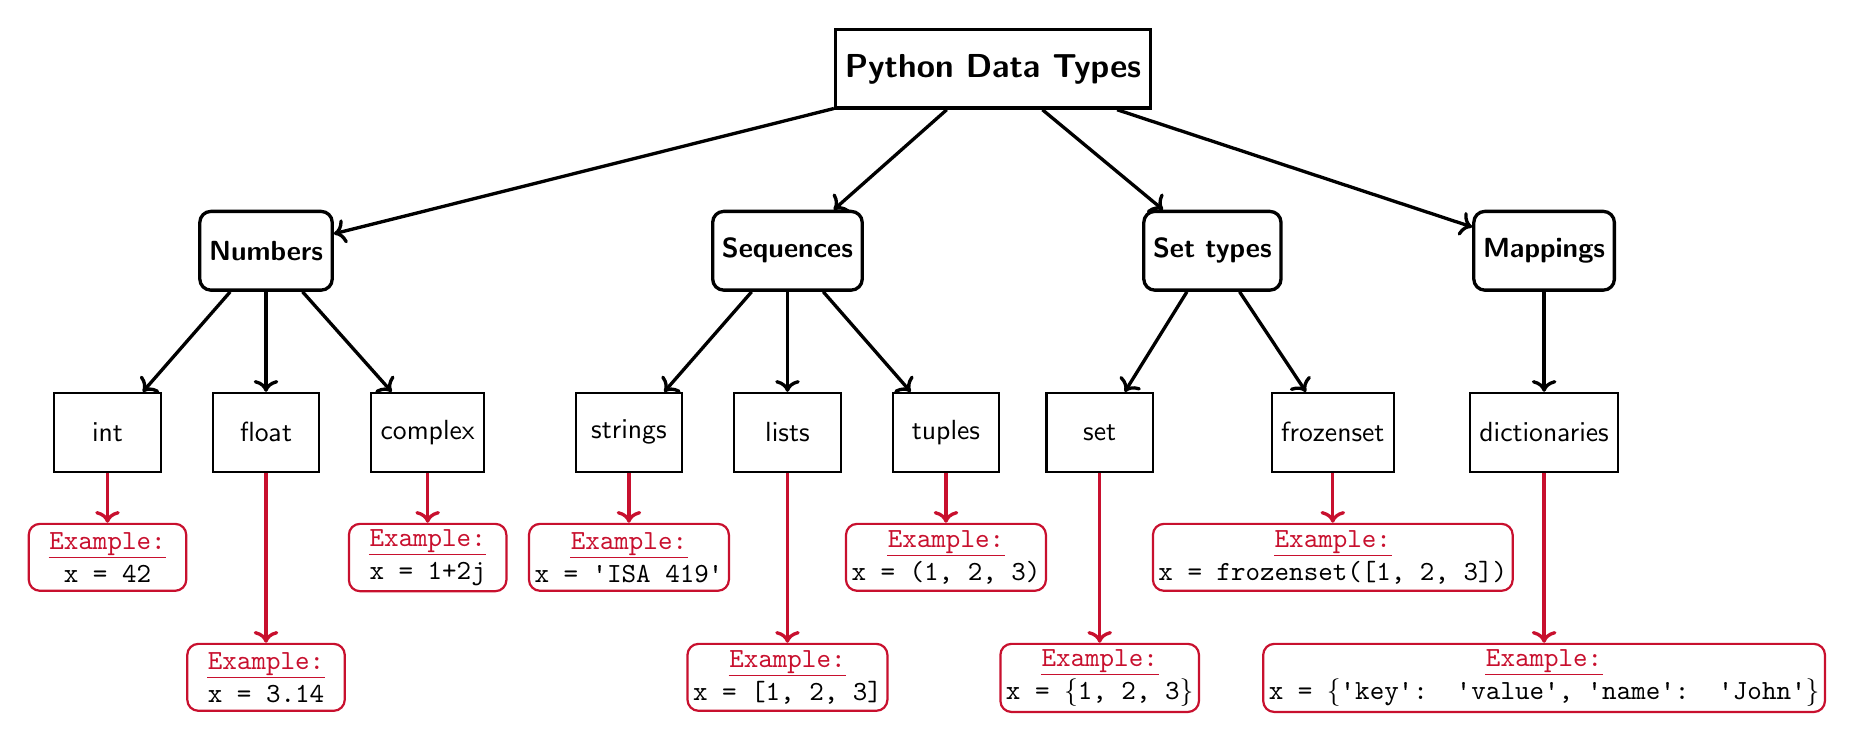
\begin{tikzpicture}

  % Level 0: Python - Data Types/Classes
  \node (data_types) [level0] {\large{Python Data Types}};

  % Level 1: None, Numbers, Sequences, Set types, Mappings, Callables/Modules/etc

  
  \node (sets) [level1, below right=0.5in and -0.05in of data_types] {Set types};

  \node (numbers) [level1, below left=0.5in and 2.5in of data_types] {Numbers};
  % \node (none) [level1, left=3in of sets] {None};
  \node (sequences) [level1, below left=0.5in and -0.15in of data_types] {Sequences};
  
  \node (mappings) [level1, below right=0.5in and 1.6in of data_types] {Mappings};
  % \node (callables) [level1, right=3in of sets] {Callables};
  % \node (modules) [level1, right=4.5in of sets] {modules};

  % Level 2: Boxes under Numbers, Sequences, Set types, Mappings
  \node (float) [level2, below=0.5in of numbers] {float};
  \node (int) [level2, left=0.25in of float] {int};
  \node (complex) [level2, right=0.25in of float] {complex};

  \node (lists) [level2, below=0.5in of sequences] {lists};
  \node (strings) [level2, left=0.25in of lists] {strings};
  \node (tuples) [level2, right=0.25in of lists] {tuples};

  \node (set) [level2, below left =0.5in and -0.15cm of sets] {set};
  \node (frozenset) [level2, below right =0.5in and -0.15cm of sets] {frozenset};

  \node (dictionaries) [level2, below=0.5in of mappings] {dictionaries};

  % Level 3: Examples
  % \node (none_example) [level3, below=1.75in of none] {\textcolor{miamired}{\ul{Example:}}\\ x = None };

  \node (int_example) [level3, below=0.25in of int] {\textcolor{miamired}{\ul{Example:}}\\ x = 42 };
  \node (float_example) [level3, below=0.85in of float] {\textcolor{miamired}{\ul{Example:}}\\ x = 3.14 };
  \node (complex_example) [level3, below=0.25in of complex] {\textcolor{miamired}{\ul{Example:}}\\ x = 1+2j };

  \node (strings_example) [level3, below=0.25in of strings] {\textcolor{miamired}{\ul{Example:}}\\ x = \textquotesingle ISA 419\textquotesingle };
  \node (tuples_example) [level3, below=0.25in of tuples] {\textcolor{miamired}{\ul{Example:}}\\ x = (1, 2, 3) };
  \node (lists_example) [level3, below=0.85in of lists] {\textcolor{miamired}{\ul{Example:}}\\ x = [1, 2, 3] };

  \node (set_example) [level3, below=0.85in of set] {\textcolor{miamired}{\ul{Example:}}\\ x = \{1, 2, 3\} };
  \node (frozenset_example) [level3, below=0.25in of frozenset] {\textcolor{miamired}{\ul{Example:}}\\ x = frozenset([1, 2, 3]) };

  \node (dictionaries_example) [level3, below=0.85in of dictionaries] {\textcolor{miamired}{\ul{Example:}}\\ x = \{\textquotesingle key\textquotesingle: \textquotesingle value\textquotesingle,  \textquotesingle name\textquotesingle: \textquotesingle John\textquotesingle\}};

  % Connect nodes with arrows
  % \draw[->, thick] (data_types) -- (none);
  \draw[->, very thick] (data_types) -- (numbers);
  \draw[->, very thick] (data_types) -- (sequences);
  \draw[->, very thick] (data_types) -- (sets);
  \draw[->, very thick] (data_types) -- (mappings);
  % \draw[->, thick] (data_types) -- (callables);
  % \draw[->, thick] (data_types) -- (modules);

  \draw[->, very thick] (numbers) -- (int);
  \draw[->, very thick] (numbers) -- (float);
  \draw[->, very thick] (numbers) -- (complex);

  \draw[->, very thick] (sequences) -- (strings);
  \draw[->, very thick] (sequences) -- (tuples);
  \draw[->, very thick] (sequences) -- (lists);

  \draw[->, very thick] (sets) -- (set);
  \draw[->, very thick] (sets) -- (frozenset);

  \draw[->, very thick] (mappings) -- (dictionaries);

  \draw[->, miamired, very thick] (dictionaries) -- (dictionaries_example);
  % \draw[->, miamired, very thick] (none) -- (none_example);
  \draw[->, miamired, very thick] (int) -- (int_example);
  \draw[->, miamired, very thick] (float) -- (float_example);
  \draw[->, miamired, very thick] (complex) -- (complex_example);
  \draw[->, miamired, very thick] (strings) -- (strings_example);
  \draw[->, miamired, very thick] (tuples) -- (tuples_example);
  \draw[->, miamired, very thick] (lists) -- (lists_example);
  \draw[->, miamired, very thick] (set) -- (set_example);
  \draw[->, miamired, very thick] (frozenset) -- (frozenset_example);
\end{tikzpicture}
\end{document}
